% ------------------------------------------------------------%
% 2015-2021 - Emerson Ribeiro de Mello <mello@ifsc.edu.br>
% ------------------------------------------------------------%
% Sets aspect ratio to 4:3, and frame size to 128 mm by 96 mm
\documentclass[aspectratio=169]{beamer}
% Sets aspect ratio to 16:9, and frame size to 160 mm by 90 mm.
% \documentclass[aspectratio=169]{beamer}
% Sets aspect ratio to 16:10, and frame size to 160 mm by 100 mm.
% \documentclass[aspectratio=1610]{beamer}
\usepackage[dvipsnames]{xcolor}
\usepackage{colortbl}
\usepackage{makecell}
\usepackage{multicol}
\usepackage{pifont}

\definecolor{DarkCyan}{HTML}{119DA4}
\definecolor{Asparagus}{HTML}{6DA34D}
\definecolor{CambridgeBlue}{HTML}{8FBC94}
\definecolor{TeaGreen}{HTML}{C5E99B}
\definecolor{Saphire}{HTML}{4059AD}



% -------------------------------------------------%
%  Package options
% -------------------------------------------------%
%  002625, EEE5E9, 0D1821, ADF7B6, B6C454
% textbgcolor   - frametitle background color. default: 0d4f4d
% textfgcolor   - frametitle foreground color. default: ffffff
% slidebgcolor  - slide background color. default: eef1ec
% slidefgcolor  - slide text foreground color. default: 000000
% authorfgcolor - author, institute and date color. default: 000000
% itemsep - space between items (itemize, enumerate). default: 7pt
\usepackage[textbgcolor=344966,textfgcolor=ffffff,slidebgcolor=EEE5E9,itemsep=7pt]{../0-ifscyan-modelo/beamerthemeifscyan}
% -------------------------------------------------%

% A good place to get some colors
% https://material.io/resources/color/#!/?view.left=0&view.right=0&primary.color=0d4f4d
% cyan: #0D4F4D, light: #417b79,  dark: #002625
% IFSC green: normal: #32A041, light: #69d26f, dark: #007013
% IFSC red: normal: #C8191E, light: #ff5747, dark: #8f0000 
% Other colors for textbgcolor
% purple 4527a0, blue 0d47a1, grey 546e7a, redwine 880e4f, brown 6d4c41, yelllow (bg=#fbc02d, fg=000000)

% Logo
\pgfdeclareimage[height=.3\paperheight]{ifpilogo}{../0-ifscyan-modelo/figs/Logo-IFPI-Vertical.png}

\AtBeginSection[]{
  \begin{frame}
  \vfill
  \centering
  \begin{beamercolorbox}[sep=8pt,center,shadow=true,rounded=true]{title}
    \usebeamerfont{title}\insertsectionhead\par%
  \end{beamercolorbox}
  \vfill
  \end{frame}
}

% -------------------------------------------------%
%              Título 
% -------------------------------------------------%
\title{Matemática Computacional}
\subtitle{Análise Combinatória}
\author{Prof. Rogério Figueredo de Sousa}
\institute{%
\href{rogerio.sousa@ifpi.edu.br}{rogerio.sousa@ifpi.edu.br}%
}%
\date{27/08/2024}
% -------------------------------------------------%

% -------------------------------------------------%
%  Início do documento 
% -------------------------------------------------%
\begin{document}

\begin{frame}[plain]
    \titlepage
\end{frame}

%\begin{frame}[plain, noframenumbering]{Licenciamento}
%    \licenciamentoLivre
%\end{frame}

%\begin{frame}[plain, noframenumbering]{Sumário}
%   \tableofcontents
%\end{frame}


\jsonp
\lstset{
    numbers=none,
    escapeinside={\%*}{*)},
}

%1
\begin{frame}{Princípio Aditivo e Multiplicativo}

    Objetivos:

    \vspace{4mm}
    \begin{itemize}
        \item Desenvolver as idéias e técnicas básicas para problemas de contagem.
        \item Reduzir um problema grande a vários problemas pequenos, usando os Princípios Aditivo e Multiplicativo.
    \end{itemize}

\end{frame}

%2
\begin{frame}{Princípio Aditivo e Multiplicativo}

    Importância:

    \vspace{4mm}
    \begin{itemize}
        \item Os problemas de contagem aparecem naturalmente no nosso dia a dia.
        \item Muitas vezes estamos apenas interessados em contar os elementos de um determinado conjunto, sem enumerá-los.
        \item No desenvolvimento de técnicas de contagem que veremos mais adiante, tais como: permutações, combinações, etc, estaremos usando basicamente os \textbf{Princípios Aditivo e Multiplicativo}.
    \end{itemize}

\end{frame}

%3
\begin{frame}{Princípio Aditivo e Multiplicativo}
    \textbf{Problemas de contagem:}

    \vspace{4mm}

  \textbf{  Exemplo 1:}

    \vspace{3mm}
    \begin{itemize}
        \item Dados quatro livros distintos de \textbf{Matemática (M1,M2,M3,M4)} e três livros distintos de \textbf{Português (P1,P2,P3)}, de quantas maneiras podemos selecionar (escolher):
        
        \vspace{3mm}
        \begin{enumerate}[a]
            \item Um livro (\underline{ou} de Matemática \underline{ou} de Português).
            \item Dois livros, sendo \underline{um} de Matemática \underline{e outro} de Português.
        \end{enumerate}
    
        
    \end{itemize}

\end{frame}

\begin{frame}{Princípio Aditivo e Multiplicativo}
    \textbf{Exemplo 1 (continuação):}

    \vspace{3mm}

    \begin{enumerate}[a]
        \item \textbf{Um livro (\underline{ou} de Matemática \underline{ou} de Português)}
    \end{enumerate}
        
    O livro de Matemática pode ser escolhido de 4 maneiras:
    \begin{itemize}
        \item livro $M_1$ ou 
        \item livro $ M_2 $ ou
        \item livro $ M_3 $ ou
        \item livro $M_4$
    \end{itemize}
    
    
    O livro de Português pode ser escolhido de 3 maneiras:

    \begin{itemize}
        \item $P_1$ ou
        \item $P_2 $ ou 
        \item $ P_3$
    \end{itemize}
    
    
    Número de maneiras: $4 + 3 = 7$
\end{frame}

\begin{frame}{Princípio Aditivo e Multiplicativo}
    \textbf{Exemplo 1 (continuação):}

    \vspace{3mm}

    \begin{enumerate}[a]
        \item \textbf{Dois livros, sendo \underline{um} de Matemática \underline{e outro} de Português.}
    \end{enumerate}

    \vspace{3mm}

    Temos dois conjuntos:

    \begin{center}
        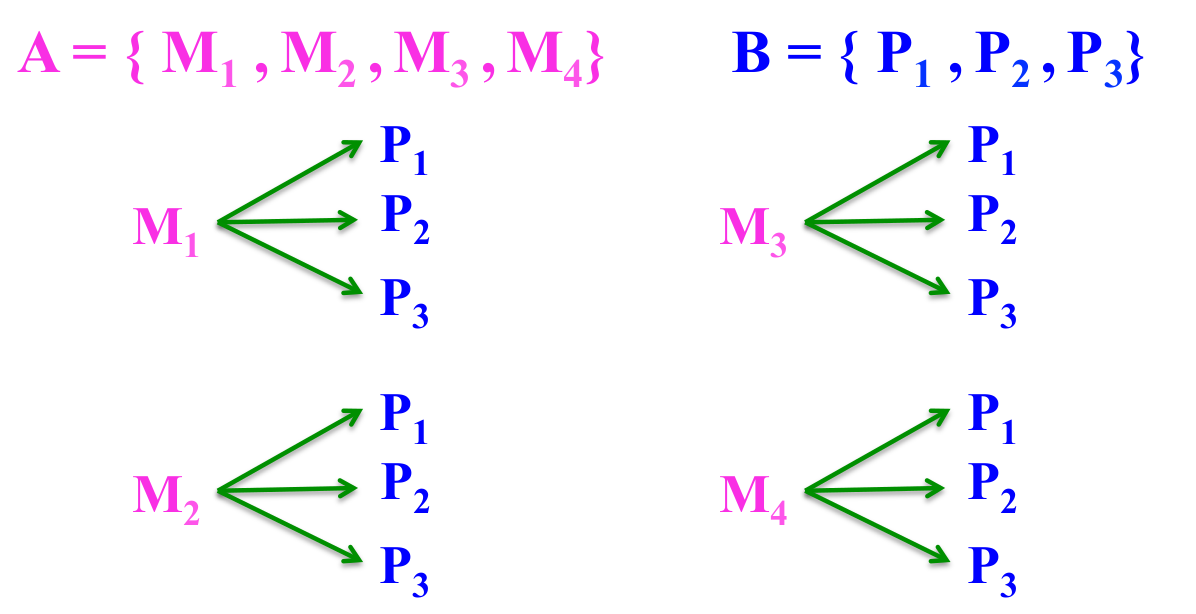
\includegraphics[width=0.65\textwidth]{figs/combinacoes_livros.png}
    \end{center}
\end{frame}

\begin{frame}{Princípio Aditivo e Multiplicativo}
    \textbf{Resumindo}

    \vspace{4mm}

    \begin{enumerate}[a]
        \item De quantas maneira podemos escolher \underline{um} livro qualquer (ou de Matemática ou de Português)?
    \end{enumerate}

    \textbf{Resposta:}

    \vspace{3mm}

    \begin{itemize}
        \item Temos 4 maneiras de escolher um livro de Matemática e 3 maneiras de escolher um livro de Português.
        \item Logo, temos $\boldsymbol{4+3=7}$ maneiras de escolher um livro qualquer dentre os de Matemática e Português.
    \end{itemize}
\end{frame}

\begin{frame}{Princípio Aditivo e Multiplicativo}
    \begin{enumerate}[a]
        \item De quantas maneira podemos escolher dois livros sendo \underline{um} de \underline{Matemática} e \underline{outro} de \underline{Português}?
    \end{enumerate}
    
    \vspace{3mm}

    \textbf{Resposta:}

    \vspace{3mm}

    \begin{itemize}
        \item Para cada livro de Matemática, temos 3 maneiras de escolher os livros de Português.
        \item Como temos 4 maneiras de escolher os livros de Matemática, teremos $ \boldsymbol{3 \times 4 = 12}$ maneiras de escolher um livro de matemática e outro de Português.
    \end{itemize}
\end{frame}


\begin{frame}{Princípio Aditivo e Multiplicativo}

    \textbf{Exemplo  2:}

    \vspace{4mm}
    Maria vai a uma papelaria para comprar \textbf{lapiseira} e \textbf{borracha}. Nessa papelaria há \textbf{7} tipos diferentes de lapiseiras e \textbf{5} tipos diferentes de borrachas.

    \vspace{3mm}

    \begin{enumerate}[a]
        \item Se o dinheiro de Maria só dá para comprar um item, ou uma lapiseira ou uma borracha, de quantas maneiras diferentes ela pode fazer isso?
    \end{enumerate}

    \begin{center}
        \begin{multicols}{2}
            $L = \{L_1, L_2, ..., L_7\}$
    
            \columnbreak
    
            $B = \{B_1, B_2, ..., B_5\} $
    
        \end{multicols}
    \end{center}

\begin{center}
    ou $L_1$, ou $L_2$, ou ... ou $L_7 \rightarrow $  7 maneiras
    
    ou $B_1$, ou $B_2$, ou ... ou $B_5 \rightarrow $  5 maneiras
    
\end{center}

Número de maneiras de escolher um item: $\boldsymbol{7 + 5 = 12}$
\end{frame}

\begin{frame}{Princípio Aditivo e Multiplicativo}

    \textbf{Exemplo  2 (continuação):}

    \vspace{3mm}
    \begin{enumerate}[b]
        \item Suponha agora que Maria tem dinheiro para comprar 2 itens, sendo que ela quer uma lapiseira e uma borracha. De quantas maneiras diferentes ela pode fazer isso?
    \end{enumerate}

    \begin{center}
        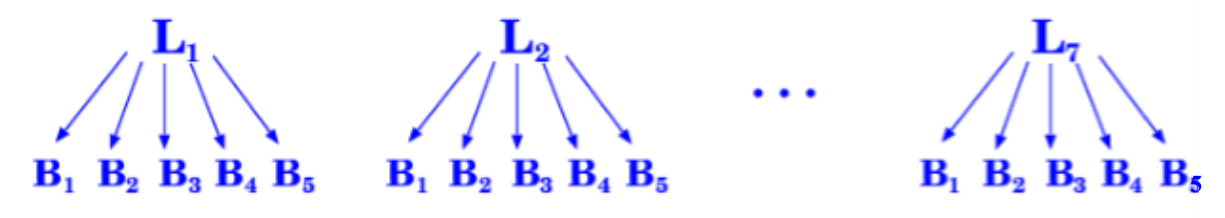
\includegraphics[width=0.8\linewidth]{figs/combinacoes_maria.png}
    \end{center}

    \vspace{2mm}

    Observe que temos os pares:

    \vspace{2mm}

    $$(L_1, B_1) (L_1, B_2) ... (L_1, B_5), ... , (L_7, B_1), (L_7, B_2), ... , (L_7, B_5)$$

    \vspace{2mm}
Número de maneiras de escolher 2 itens, sendo um item uma lapiseira e outro uma borracha: $\boldsymbol{5 + 5 + ... + 5 = 5 \times 7 = 35}$
\end{frame}


\begin{frame}{Princípio Aditivo e Multiplicativo}
\textbf{Resumindo}

\begin{enumerate}[a]
    \item De quantas maneiras diferentes Maria pode comprar um item (ou um lapiseira ou um borracha)?
\end{enumerate}

\vspace{4mm}
\textbf{Resposta:}

\begin{itemize}
    \item[] Ela tem 7 possibilidades de escolha de lapiseira e 5 possibilidades de escolha de borracha.
    \item[] Logo, Maria tem \textbf{7 + 5} possibilidades diferentes de comprar \underline{ou} uma lapiseira \underline{ou} uma borracha. 
\end{itemize}

\end{frame}


\begin{frame}{Princípio Aditivo e Multiplicativo}
     \begin{enumerate}[b]
        \item De quantas maneiras diferentes Maria pode comprar 2 itens: uma  lapiseira \underline{e} uma borracha?
    \end{enumerate}
    
    \vspace{4mm}
    \textbf{Resposta:}
    
    \begin{itemize}
        \item[] Para cada escolha de lapiseira, ela tem 5 escolhas de borracha.
        \item[] Como ela tem 7 escolhas de lapiseiras diferentes, ela terá $7 \times 5$ maneiras diferentes de comprar uma lapiseira e uma borracha.
    \end{itemize}
    
    \end{frame}

\begin{frame}{Introdução ao Princípio Aditivo (PA)}
    \begin{itemize}
        \item \textbf{Princípio Aditivo} (para dois conjuntos)
        \item[] \underline{Se} A e B são dois conjuntos disjuntos $(A \cap B = \emptyset)$,
        \item[] \underline{então} $n(A \cup B) = n(A) + n(B)$
    \end{itemize}

    \vspace{4mm}

    \begin{itemize}
        \item Outra notação usual
        \begin{itemize}
            \item[] $n(A) = |A|$
            \item[] $n(B) = |B|$
            \item[] $n(A \cup B) = |A \cup B| = |A| + |B| $
        \end{itemize}
    \end{itemize}
\end{frame}


\begin{frame}{Introdução ao Princípio Aditivo (PA)}
    \begin{itemize}
        \item Outra interpretação da formulação:
        \begin{itemize}
            \item Sejam \textbf{A} e \textbf{B} eventos mutuamente exclusivos. Se um evento \textbf{A} pode ocorrer de \textbf{m} maneiras e outro evento \textbf{B} pode ocorrer de \textbf{n} maneiras, então existem $m + n$ maneiras em que algum desses dois eventos podem ocorrer. 
        \end{itemize}
    \end{itemize}
\end{frame}

\begin{frame}{Introdução ao Princípio Aditivo (PA)}
    \textbf{Voltando ao exemplo 1:}

    \vspace{4mm}
    \begin{itemize}
        \item Dados quatro livros distintos de Matemática e três livros distintos de Português:
        \begin{enumerate}[a]
            \item De quantas maneiras podemos escolher um livro qualquer?
        \end{enumerate}
    \end{itemize}

    \vspace{3mm}
    Podemos identificar os conjuntos:
    \begin{center}
        \begin{multicols}{2}
            $A = \{ M1, M2, M3, M4 \} $
            
            \columnbreak
    
            $B = \{ P1, P2, P3 \}$    
        \end{multicols}
    \end{center}

    % \vspace{2mm}

    \begin{center}
        \begin{multicols}{3}
            $A \cap B= \emptyset $ 

            \columnbreak

            $|A| = n(A) = 4$

            \columnbreak

            $|B| = n(B) = 3$
        \end{multicols}
    \end{center}

    \begin{itemize}
        \item Pelo P. A. temos
        \begin{itemize}
            \item[] $|A \cup B| = |A| + |B| = 7$ maneiras de escolher um livro qualquer, ou de Matemática ou de Português. 
        \end{itemize}
    \end{itemize}
\end{frame}


\begin{frame}{Introdução ao Princípio Aditivo (PA)}
    \textbf{Voltando ao exemplo 2:}

    \vspace{4mm}
    \begin{itemize}
        \item Na papelaria há 7 tipos diferentes de lapiseira e 5 tipos diferentes de borracha:
        \begin{enumerate}[a]
            \item De quantas maneiras Maria pode comprar um item?
        \end{enumerate}
    \end{itemize}

    \vspace{3mm}
    Identificando os conjuntos:
    \begin{center}
        \begin{multicols}{2}
            $L = \{L1, L2, ..., L\}$
            
            \columnbreak
    
            $B = \{B1, B2, ..., B5\}$    
        \end{multicols}
    \end{center}

    % \vspace{2mm}

    \begin{center}
        \begin{multicols}{3}
            $L \cap B = \emptyset$ 

            \columnbreak

            $|L| = 7$

            \columnbreak

            $|B| = 5$
        \end{multicols}
    \end{center}

    \begin{itemize}
        \item Pelo P. A., Maria tem
        \begin{itemize}
            \item[] $|L \cup B| = |L| + |B| = 7 + 5 = 12$ maneiras de escolher ou uma lapiseira ou uma borracha. 
        \end{itemize}
    \end{itemize}
\end{frame}

\begin{frame}{Introdução ao Princípio Multiplicativo (PM)}
\begin{itemize}
    \item Princípio Multiplicativo (para dois conjuntos)
    \item[] Se A é um conjunto com m elementos e B é um conjunto com n elementos então o conjunto $A \times B$
\end{itemize}

\begin{center}
    $$A \times B = \{(a, b) | a \in A ~ e ~ b \in B\}$$
    
    tem $m \times n$ elementos
    
    $$|A \times B| = |A| . |B| =  m \times n$$
\end{center}
\end{frame}


\begin{frame}{Introdução ao Princípio Multiplicativo (PM)}
\begin{itemize}
    \item Outra interpretação da formulação:
    \begin{itemize}
        \item Se um evento A pode ocorrer de m maneiras e um evento B pode ocorrer de n maneiras então o par de eventos, primeiro um e depois o outro, podem ocorrer de $m \times n$ maneiras.
    \end{itemize}
    
\end{itemize}
\end{frame}

%18
\begin{frame}{Introdução ao Princípio Multiplicativo (PM)}
    \textbf{Voltando ao exemplo 1:}

    \vspace{4mm}
    \begin{itemize}
        \item Dados quatro livros distintos de Matemática e três livros distintos de Português:
        \begin{enumerate}[b]
            \item De quantas maneiras podemos escolher 2 livros sendo um de Matemática e outro de Português?
        \end{enumerate}
    \end{itemize}

    \vspace{2mm}
    Identificando os conjuntos:
    \begin{center}
        \begin{multicols}{2}
            $A = \{M_{1}, M_{2}, M_{3}, M_{4}\}$
            
            \columnbreak
    
            $B = \{P_{1}, P_{2}, P_{3}\}$    
        \end{multicols}
    \end{center}

    % \vspace{2mm}

    \begin{center}
        \begin{multicols}{2}
            $|A| = 4$ 

            \columnbreak

            $|B| = 3$
        \end{multicols}
    \end{center}

    \begin{itemize}
        \item Pelo P.M. temos então:
        \begin{itemize}
            \item[] $\boldsymbol{|A \times B| = |A| \times |B| = 4 \times 3 = 12}$ maneiras de escolher dois livros sendo um de Matemática e outro de Português.
        \end{itemize}
    \end{itemize}

    \vspace{2mm}
    Exercício: Interpretação do exercício 2 b).

\end{frame}

%19
\begin{frame}{Introdução ao Princípio Multiplicativo (PM)}
    \textbf{Exemplo 3:}

    \vspace{2mm}
    \begin{itemize}
        \item Um prédio tem oito portas:
        \begin{enumerate}[a]
            \item De quantas maneiras uma pessoa pode entrar e sair?
        \end{enumerate}
    \end{itemize}

    \vspace{2mm}
       
    \begin{center}
        \begin{multicols}{2}
            $A = B = \{ P_1, P_2, ..., P_8 \}$
            
            \columnbreak
    
            $|A| = 8$    
        \end{multicols}
    \end{center}

    \begin{center}
        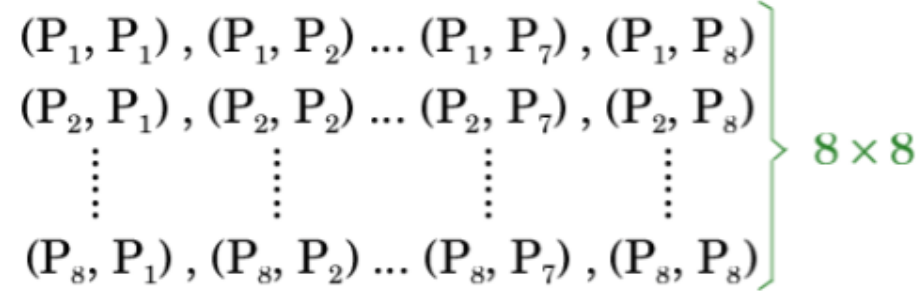
\includegraphics[width=0.5\linewidth]{figs/combinacoes_portas.png}
    \end{center}
    % \vspace{2mm}

    \begin{center}
        $|A \times B| = |A| \times |A| = 8 \times 8 = 64$
    \end{center}

    Resposta:

    \vspace{3mm}
    \begin{itemize}
        \item Uma pessoa pode entrar e sair do prédio de 64 maneiras.
    \end{itemize}

\end{frame}

%20
\begin{frame}{Introdução ao Princípio Multiplicativo (PM)}
    \textbf{Exemplo 3 (continuação):}

    \vspace{2mm}

        \begin{enumerate}[b]
            \item De quantas maneiras uma pessoa pode entrar por uma
            porta e sair por outra diferente?
            \item[] Observe: Se usarmos a porta $P_1$ para entrar, ela não pode
            ser usada para sair.
        \end{enumerate}

    \vspace{2mm}
   

    \begin{center}
        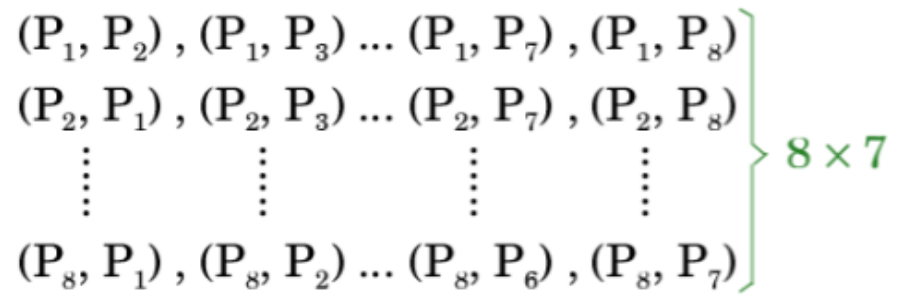
\includegraphics[width=0.5\linewidth]{figs/combinacoes_portas2.png}
    \end{center}
    % \vspace{2mm}

    Resposta:

    \vspace{3mm}
    \begin{itemize}
        \item Uma pessoa pode entrar por uma porta e sair por uma
        outra diferente de 56 maneiras.
    \end{itemize}

\end{frame}


%21
\begin{frame}{Introdução ao Princípio Multiplicativo (PM)}
    \textbf{Exemplo 3 (continuação):}

    \vspace{2mm}

        \begin{enumerate}[b]
            \item Formalização:
            \item[] $A = \{ P_1, P_2, ..., P_8\}, |A| = 8 $
            \item[] $D = \{ (P_1, P_1), ..., (P_8, P_8) \}, |D| = 8$
            \item[] $C=A \times A - D$
        \end{enumerate}

    \vspace{2mm}
   

    \begin{center}
        \begin{multicols}{2}
            $|C| = |A \times A| - |D|$

            $|C| = |A| . |A|-|D|$
            \columnbreak

            (Princípio Aditivo)

            (Princípio Multiplicativo)
        \end{multicols}
    \end{center}
    % \vspace{2mm}

    \vspace{3mm}
    \begin{itemize}
        \item[] $= 8 \times 8 - 8 = 8(8 - 1) = 8 ~ .~  7$
    \end{itemize}
    

\end{frame}


%22
\begin{frame}{Introdução ao Princípio Multiplicativo (PM)}
    \textbf{Exemplo 3 (continuação):}

    \vspace{2mm}
        \begin{itemize}
            \item Interpretação:
            \begin{enumerate}[a]
                \item De quantas maneiras uma pessoa pode entrar e sair?
                
                \begin{multicols}{2}
                    \begin{itemize}
                        \item[] Maneiras de entrar - 8
                        \item[] Maneiras de sair - 8
                    \end{itemize}
                    \columnbreak

                    $8 \times 8 = 64$
                \end{multicols}

                \item De quantas maneiras uma pessoa pode entrar por uma porta e sair por outra diferente?
                
                \begin{multicols}{2}
                    \begin{itemize}
                        \item[] Maneiras de entrar - 8
                        \item[] Maneiras de sair - 7
                    \end{itemize}
                    \columnbreak

                    \vspace{2mm}

                    $8 \times 7 = 56$
                \end{multicols}
            \end{enumerate}
        \end{itemize}
\end{frame}


%23
\begin{frame}{Introdução ao Princípio Multiplicativo (PM)}
    \textbf{Exemplo 4:}

    \vspace{2mm}
        \begin{itemize}
            \item Numa sala estão reunidos cinco homens, seis mulheres e quatro crianças.
            \item De quantas maneiras podemos selecionar:
            \begin{enumerate}[a]
                \item Uma pessoa?
                \item um homem, uma mulher e uma criança?
            \end{enumerate}
        \end{itemize}
\end{frame}

%24
\begin{frame}{Introdução ao Princípio Multiplicativo (PM)}
    \textbf{Exemplo 4 (continuação):}

    \vspace{2mm}
        \begin{enumerate}[a]
                \item De quantas maneiras podemos selecionar uma pessoa?
                \item[] $H = \{ h_1, h_2, h_3, h_4, h_5 \}$
                \item[] $M = \{ m_1, m_2, m_3, m_4, m_5, m_6 \}$
                \item[] $C = \{ C_1, C_2, C_3, C_4 \}$
        \end{enumerate}

    \vspace{2mm}
    \begin{center}
        \begin{multicols}{3}
            $H \cap M = \emptyset $

            $|H|=5$

            \columnbreak

            $H \cap C = \emptyset $

            $|M| = 6 $

            \columnbreak

            $M \cap C = \emptyset$

            $|C| = 4$

        \end{multicols}
    \end{center}

    $$|H \cup M \cup C| = |H| \cup |M| \cup |C| = 5 + 6 + 4 = 15$$

    $$H \cup M \cup C = { h_1, h_2, ..., h_5, m_1, m_2, ..., m_6, c_1, ..., c_4}$$

\end{frame}

%25
\begin{frame}{Introdução ao Princípio Multiplicativo (PM)}
    \textbf{Exemplo 4 (continuação):}

    \vspace{2mm}
        \begin{enumerate}[a]
                \item De quantas maneiras podemos selecionar um homem,
                uma mulher e uma criança?
        \end{enumerate}

    \vspace{2mm}

    $$H \times M \times C = \{ (h,m,c) ~| ~ h \in H, m \in M, c \in C\}$$

    \vspace{2mm}

\begin{center}
        $\textbf{H} \times \textbf{M} \times \textbf{C} = \{(h_1, m_1, c_1), (h_1, m_2, c_1), (h_1, m_3, c_1),$ \\
    $\quad \quad \quad \quad \quad \quad ~ ~ ~ (h_1, m_4, c_1), (h_1, m_5, c_1), (h_1, m_6, c_1),$ \\
    $\quad \quad \quad \quad \quad \quad \quad \quad \quad ~  (h_1, mb_1, c_2), (h_1, m_1, c_3), (h_1, m_1, c_4), \dots \}$
    
\end{center}

   \begin{itemize}
    \item Observação
    \begin{itemize}
        \item[] $|H \times M \times C| = |H| \times |M| \times |C| = 5 \times 6 \times 4 = 120$
    \end{itemize}
   \end{itemize}

\end{frame}

\begin{frame}{Extensão do Princípio Aditivo}
\begin{itemize}
    \item Se $A_1, A_2, ... A_n$ são conjuntos disjuntos dois a dois
\end{itemize}

$$(A_i \cap A_j = \emptyset \quad i \neq j)$$ 

$$ e ~ |A_1| = m_1, |A_2| = m_2, ..., |A_n| = m_n$$

\vspace{4mm}

\begin{itemize}
    \item[] então o conjunto $\bigcup_{i = 1}^{n}  = A_1 \cup A_2 \cup ... \cup A_n$
    \item[] possui $m_1 + m_2 + ... + m_n$ elementos
\end{itemize}

$$ |A_1 \cup A_2 \cup ... \cup A_n| = |A_1| + |A_2| + ... + |A_n| = \sum_{i=1}^{n} m_i$$
\end{frame}

%28
\begin{frame}{Extensão do Princípio Aditivo}
\begin{itemize}
    \item Outra interpretação da formulação:
    \item[] Sejam $A_1, A_2, ..., A_n$ eventos mutuamente exclusivos. Se cada evento $A_i$ pode ocorrer de $m_i$ maneiras então existem $m_1 + m_2 + ... + m_n$ maneiras em que algum desses n eventos podem ocorrer.
\end{itemize}
\end{frame}

%29
\begin{frame}{Extensão do Princípio Multiplicativo}
    \begin{itemize}
        \item Sejam $A_1, A_2, ... A_n$ conjuntos tais que
    \end{itemize}
    
    $$ |A_1| = m_1, |A_2| = m_2, ..., |A_n| = m_n$$
    
    \vspace{4mm}
    
    \begin{itemize}
        \item[] então o conjunto $\prod_{i = 1}^{n} A_i = A_1 \times A_2 \times ... \times A_n$
        \item[] possui $m_1 \times m_2 \times ... \times m_n$ elementos
    \end{itemize}
    
    $$ |A_1 \times A_2 \times ... \times A_n| = |A_1| \times |A_2| \times ... \times |A_n| = \prod_{i=1}^{n} m_i$$
    \end{frame}

    %30
\begin{frame}{Extensão do Princípio Multiplicativo}
    \begin{itemize}
        \item Outra interpretação da formulação:
        \item[] Se temos n eventos $A_1, A_2, ..., A_n$, onde cada evento $A_i$ pode ocorrer de $m_i$ maneiras então existem $m_1 \times m_2 \times ... \times m_n$ maneiras em que esses n eventos podem ocorrer sucessivamente.
    \end{itemize}
    \end{frame}


\begin{frame}{Extensão do Princípio Aditivo}

    \textbf{Exemplo 5:}

\begin{itemize}
    \item Uma bandeira é formada por três listras que devem ser coloridas usando-se apenas as cores: amarelo, branco, azul, de tal maneira que listras adjacentes não recebam a mesma cor.
    \item[] De quantos modos podemos colorir esta bandeira?
\end{itemize}

\begin{center}
    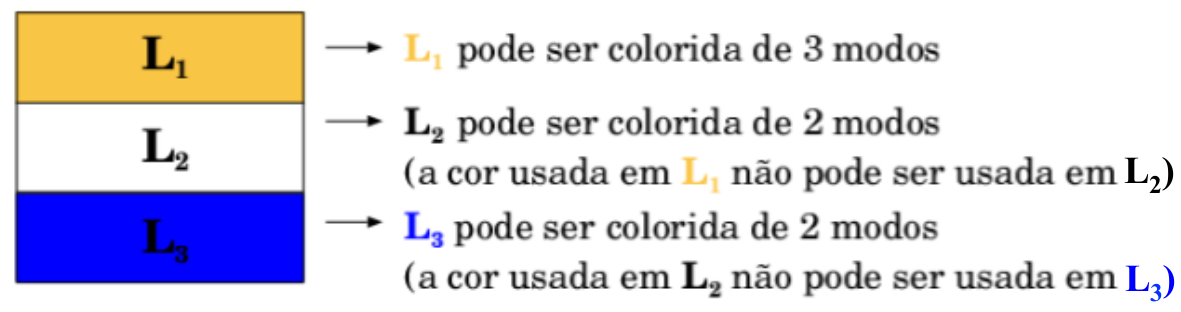
\includegraphics[width=0.9\linewidth]{figs/bandeira.png}
\end{center}

Logo pelo PM temos $3 \times 2 \times 2$ modos de colorir esta bandeira.
\end{frame}

%31
\begin{frame}{Extensão do Princípio Aditivo}

    \textbf{Exemplo 6:}

\begin{itemize}
    \item Um teste de matemática consta de 20 perguntas para
    serem classificadas como Verdadeiras ou Falsas.
    
    \item[] Quantos são os possíveis gabaritos para este teste?
\end{itemize}

\vspace{3mm}
Resposta:

\begin{itemize}
    \item[] Cada pergunta tem duas possibilidades de resposta:
    \item[] Verdadeiro ou Falso 
\end{itemize}

\begin{center}
    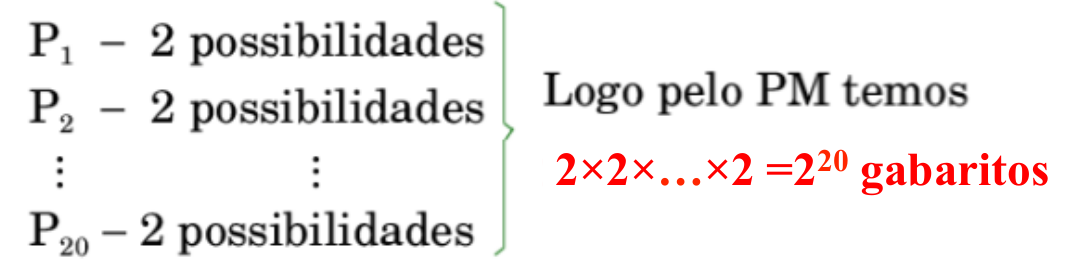
\includegraphics[width=0.8\linewidth]{figs/perguntas.png}
\end{center}
\end{frame}


%31
\begin{frame}{Extensão do Princípio Aditivo}

    \textbf{Exemplo 7:}

\begin{itemize}
    \item Considerando os algarismos 1, 2, 3, 4, 5 e 6, quantos
    números naturais de três algarismos distintos podem ser
    formados?
    
    \vspace{4mm}
    \item[] Para formar números naturais de três algarismos, podemos considerar que temos três posições a serem preenchidas:
\end{itemize}

\vspace{3mm}

\begin{center}
    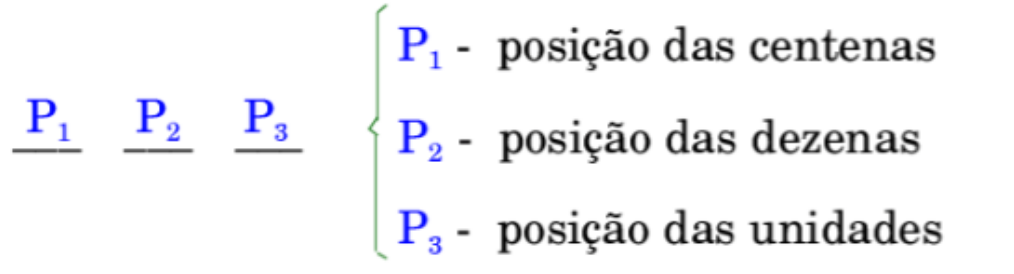
\includegraphics[width=0.8\linewidth]{figs/3digitos.png}
\end{center}
\end{frame}


%32
\begin{frame}{Extensão do Princípio Aditivo}

    \textbf{Exemplo 7 (continuação):}

\begin{itemize}
    \item Exemplo de número formado
\end{itemize}

\vspace{3mm}

\begin{center}
    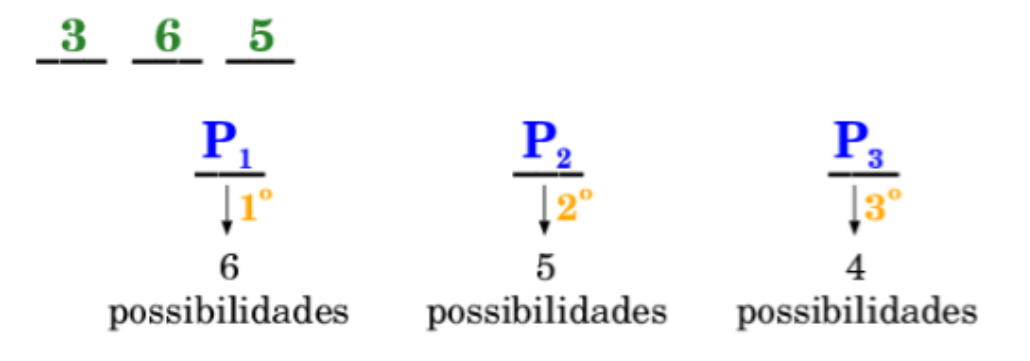
\includegraphics[width=0.8\linewidth]{figs/3digitos2.png}
\end{center}

Logo pelo PM temos $\boldsymbol{6 \times 5 \times 4 = 120}$ números naturais de três
algarismos distintos formados com os algarismos 1, 2, 3, 4, 5 e
6.
\end{frame}

%33
\begin{frame}{Extensão do Princípio Aditivo}

    \textbf{Exemplo 8:}

\begin{itemize}
    \item Quantos números naturais de três algarismos distintos (na
    base 10) existem?
    
    \vspace{3mm}
    \item[] Observação: Estamos considerando agora os algarismos $0, 1, 2, ..., 9.$
\end{itemize}

\begin{center}
    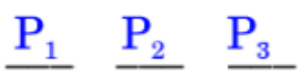
\includegraphics[width=0.3\linewidth]{figs/3digitos3.png}
\end{center}

\begin{itemize}
    \item Na posição $P_1$ temos 9 possibilidades (estamos excluindo o zero)
    \item Na posição $P_2$ temos 9 possibilidades (diferentes do anterior)
    \item Na posição $P_3$ temos 8 possibilidades (diferente dos dois anteriores) 
\end{itemize}
\vspace{2mm}

Logo pelo PM temos $\boldsymbol{9 \times 9 \times 8}$ números naturais de três algarismos
distintos.
\end{frame}


%34
\begin{frame}{Extensão do Princípio Aditivo}

    \textbf{Exemplo 8 (continuação):}

\begin{itemize}
    \item E se neste exemplo em vez de começarmos analizando a posição $P_1$, começassemos pela $P_3$?
\end{itemize}

\begin{center}
    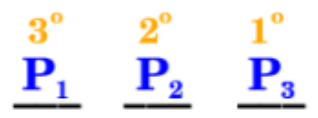
\includegraphics[width=0.25\linewidth]{figs/3digitos4.png}
\end{center}

\begin{itemize}
    \item Na posição $P_3$ temos 10 possibilidades
    \item Na posição $P_2$ temos 9 possibilidades (diferente do anterior)
    \item Na posição $P_1$ temos:
    \begin{itemize}
        \item 8 (se o algarismo zero já tiver sido usado), ou
        \item 7 (caso contrário)
    \end{itemize} 
\end{itemize}
\vspace{2mm}

\end{frame}

%35
\begin{frame}{Extensão do Princípio Aditivo}

    \textbf{Exemplo 8 (continuação):}

\begin{itemize}
    \item Quebramos o problema em dois:
\end{itemize}

\begin{enumerate}
    \item Ignoramos o fato do zero não estar na posição $P_{1}$ e contamos todas as possibilidades (com ele incluído)
\end{enumerate}

\begin{center}
    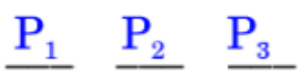
\includegraphics[width=0.25\linewidth]{figs/3digitos3.png}
\end{center}

\begin{itemize}
    \item Na posição $P_{3}$ temos 10 possibilidades
    \item Na posição $P_{2}$ temos 9 possibilidades
    \item Na posição $P_{1}$ temos 8 possibilidades
\end{itemize}
\vspace{2mm}

Logo pelo PM temos $\boldsymbol{10 \times 9 \times 8 = 720}$ números de três algarismos distintos onde o zero pode estar na posição \textbf{P}.
\end{frame}

%36
\begin{frame}{Extensão do Princípio Aditivo}

    \textbf{Exemplo 8 (continuação):}

\begin{enumerate}[2]
    \item Contamos os números de três algarismos distintos que tem apenas o zero na posição $P_1$
\end{enumerate} 

\begin{center}
    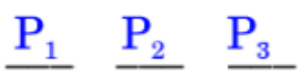
\includegraphics[width=0.25\linewidth]{figs/3digitos3.png}
\end{center}

\begin{itemize}
    \item Na posição $P_{1}$ temos 1 possibilidade
    \item Na posição $P_{2}$ temos 9 possibilidades
    \item Na posição $P_{3}$ temos 8 possibilidades
\end{itemize}
\vspace{2mm}

Logo pelo PM temos $\boldsymbol{1 \times 9 \times 8 = 72}$ números de três algarismos distintos que tem apenas o zero na posição $\boldsymbol{P_1}$.
\vspace{2mm}

Temos então $\boldsymbol{720 - 72  = 648}$ números naturais de três algarismos distintos.
\end{frame}

\end{document}